\section{Segmentation of the MILP problem}
\label{section:segment}
In this section we propose a preprocessing pipeline that makes the problem more scalable. The first step is finding an initial path with the Theta* algorithm. Note how we call this a path and not a trajectory. Unlike a trajectory, a path is not time-dependent and does not take dynamic properties into account. The second step is finding the corners in that path. The third step is generating segments based on those corners. Finally, the active obstacles to be modeled in the MILP problem are selected while the others are approximated with a genetic algorithm. \\
The goal is to segment the problem in such a way that only a minimal amount of obstacles need to be modeled in each segment, while still resulting in a relatively fast trajectory. Shorter segments with fewer obstacles are easier to solve, but the vehicle will need to travel at a lower velocity. This is because there is no information available about the next segment. If the next segment contains a tight corner, the vehicle may not be able to slow down enough if it is going too fast. Longer segments allow the vehicle to travel faster, but they need more time to solve.\\
For the best results, we want to find segments which are as large as possible but contain as few obstacles as possible. By generating a segment for each corner in the path, we can make the segments just large enough so the vehicle can always slow down in time to navigate the corner. This way the vehicle will always navigate corners  efficiently, without making the segments too large to solve in an acceptable amount of time.
\subsection{Finding the initial path}


\begin{figure}
    \centering
        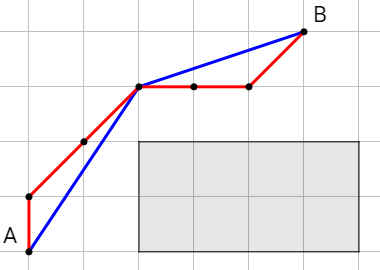
\includegraphics[width=0.6\columnwidth]{img/a_theta_star_comp2}
    \caption{A typical A* path in blue compared to a Theta* path in red. The gray rectangle is an obstacle.}\label{fig:pre-comp}
\end{figure}

\begin{figure}[!t]
    \centering
        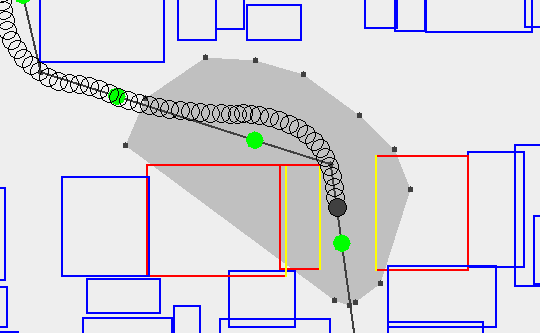
\includegraphics[width=0.8\columnwidth]{img/pre-full}
    \caption{A visualisation of the output of the algorithm The blue shapes are inactive obstacles. The red/yellow shapes are active obstacles using the same color scheme as in Fig. \ref{fig:obs-regions}. The green circles depict the transitions between segments. The dark gray shape is the convex safe area generated by the genetic algorithm. The solid black circle represents the current position of the vehicle, with the hollow circles showing the position in previous time steps.}\label{fig:pre-full}
\end{figure}
Because the trajectory is divided into segments, the vehicle cannot reach the goal immdiately and needs to be guided towards the goal.\\
One option is to simply get as close as possible to the goal during each segment. Because the distance that can be traveled during a segment is limited, the amount of obstacles that need to be modeled is also limited. This works well when the world is open with little obstacles. However, this greedy approach is prone to getting stuck in dead ends in more dense worlds like cities.\\
The second option is using an approximate path as a heuristic using an algorithm like A*. This A* path is the shortest path, but does not take constraints or the characteristics of the vehicle into account. A very curvy direct path may be the shortest, but a detour which is mostly straight and allows for higher speeds may actually be faster. \\
As always with a heuristic, there needs to be a balance between the quality and the execution time of the heuristic. A more advanced path planning algorithm could be used as the heuristic, but that will inherently also increase the execution time of the heuristic. We have decided to use Theta*. This is a variant  of A* that allows for paths at arbitrary angles instead of multiples of 45 degrees. The main reason for this is that it eliminates the artificial ``zig zags'' that A* produces. Fig. \ref{fig:pre-comp} shows a comparison between A* and Theta*.
\subsection{Detecting corner events}
With an initial path generated, the next problem is dividing it into segments. When solving each segment, the solver has no knowledge of what will happen in the next segment. This is can cause issues when the vehicle needs to make a tight corner. If the last segment ends right before the corner, it may not be possible to avoid a collision. Because of this, corners need to be taken into account when generating the segments. \\
In Euclidian geometry, the shortest path between two points is always a straight line. When polygonal obstacles are introduced between those points, the shortest path will be composed of straight lines with turns at one or more vertices of the obstacles. The obstacle that causes the turn will always be on the inside of the corner. These obstacles on the inside of the corner make the search space non-convex. For obstacles on the outside of the corner it is possible to constrain the search space so it is still convex.\\
Because of these reasons, isolating the corners from the rest of the path is advantageous. With enough buffer before the corner, the vehicle is much more likely to be able to navigate the corner successfully. It also means that the computationally expensive parts of the path are as small as possible while still containing enough information for fast navigation through the corners.\\
Because we have used Theta*, every single node in the path generated by the algorithm is guaranteed to be either the start, goal or near a corner. A corner can have more than one node, so nodes which turn in the same direction and are close to each other are grouped together and considered part of the same corner. For each corner, a corner event is generated.
\subsection{Generating path segments}
The corner events are in turn grown outwards to cover the approach and departure from the corner. The distance by which they are grown depends on the maximum acceleration of the vehicle: If the vehicle can come to a complete stop from its maximum speed before the corner, it can also successfully navigate that corner. When corners appear in quick succession, their expanded regions may overlap. In that case, the middle between those corners is chosen. Long, straight sections are also divided into smaller path segments. Fig. \ref{fig:pre-comp} shows the segment transitions as green circles.\\
One of the main goals of segmenting the path is to reduce the amount of obstacles. Every segment has a set of active obstacles associated with it, being the obstacles that need to be modeled for the solver. Not only the obstacle that ``causes'' the corner is important, but obstacles which are nearby are important as well. Obstacles on the outside of the corner also may play a role in how the vehicle approaches the corner. To find all potentially relevant obstacles, the convex hull of the (Theta*) path segment is calculated and scaled up slightly. Every obstacle which overlaps with this shape is considered an active obstacle for that path segment. The convex hull step ensures that all obstacles on the inside of the corner are included, while scaling it up will cover any restricting obstacle on the outside of the corner.
\subsection{Generating the active region for each segment}
The inactive obstacles also need to be represented. To do this, a convex polygon is constructed around the path. This polygon may intersect with the active obstacles (since they will be represented separately), but may not intersect any other obstacle. The polygon is grown using a genetic algorithm. Each individual in the population represents a single legal polygon. A legal polygon is convex, does not self-intersect, does not overlap with inactive obstacles and contains every node in the Theta* path for that specific segment. The last requirement prevents the polygon from drifting off. Each individual has a single chromosome, and each chromosome has a varying number of genes. Each gene represents a vertex of the polygon. Tournament selection is used as the selector, with the fitness function being the surface area of the polygon. No crossover operator is used. Instead, the individuals are mutated to produce a single individual as offspring each. Both the parents and offspring compete together for survival. \\
When an individual is mutated, vertices can be added, removed or nudged. The nudge mutator moves a vertex of the polygon randomly by a small amount and checks if the resulting polygon is legal. If the new polygon is legal, the mutation is kept. Otherwise the mutator tries again until the maximum amount of attempts is reached, producing no offspring. \\
The genetic algorithm is just one way to generate the convex polygon which represents the active region. Deits and Tedrake \cite{Deits2015} have demonstrated how another algorithm can solve the same problem. Fig. \ref{fig:pre-comp} Shows the active obstacles in yellow and red, as well as the polygon generated by the genetic algorithm in dark gray.

